\documentclass[]{article}
\usepackage[utf8]{inputenc}
\usepackage{multicol}
\usepackage{amsmath}
\usepackage{amsthm}
\usepackage{amssymb}
\usepackage{bm}
\usepackage{physics}
\usepackage{graphicx}
\usepackage{float}
\usepackage{caption}
\usepackage{subcaption}
%\usepackage[round]{natbib}
%\bibliographystyle{unsrtnat}

% this just sets up the page size and margins
\setlength{\topmargin}{0pt}
\setlength{\oddsidemargin}{0pt}
\setlength{\evensidemargin}{0pt}
\setlength{\textwidth}{6.5in}
\setlength{\textheight}{8.5in}
\setlength{\headheight}{0pt}

% create some short cut commands
\newcommand{\bx}{\boldsymbol{x}}
\newcommand{\by}{\boldsymbol{y}}
\newcommand{\bu}{\boldsymbol{u}}


% this is a bunch of stuff that allows python style code snippits
% Default fixed font does not support bold face
\DeclareFixedFont{\ttb}{T1}{txtt}{bx}{n}{10} % for bold
\DeclareFixedFont{\ttm}{T1}{txtt}{m}{n}{10}  % for normal
% Custom colors
\usepackage{color}
\definecolor{deepblue}{rgb}{0,0,0.5}
\definecolor{deepred}{rgb}{0.6,0,0}
\definecolor{deepgreen}{rgb}{0,0.5,0}

\usepackage{listings}

% Python style for highlighting
\newcommand\pythonstyle{\lstset{
		language=Python,
		basicstyle=\ttm,
		morekeywords={self},              % Add keywords here
		keywordstyle=\ttb\color{deepblue},
		emph={MyClass,__init__},          % Custom highlighting
		emphstyle=\ttb\color{deepred},    % Custom highlighting style
		stringstyle=\color{deepgreen},
		frame=tb,                         % Any extra options here
		showstringspaces=false,
		tabsize=4
}}

\newcommand{\mpc}{\textsc{mpc}}
\newcommand{\nmpc}{\textsc{nmpc}}

% Python environment
\lstnewenvironment{python}[1][]
{
	\pythonstyle
	\lstset{#1}
}
{}

% Python for inline
\newcommand\pythoninline[1]{{\pythonstyle\lstinline!#1!}}

\title{Comparison of Direct Methods for NMPC  Applied to  a Thrust Vector Drone}
\author{Izzy Mones and Heidi Dixon}
%\date{}

\begin{document}
	\maketitle
	
	\section*{Introduction}	
	\begin{enumerate}
		\item What is a Thrust Vector Drone and Why they are useful for Rocket Design
	\end{enumerate}
	

	
	\section*{Thrust Vector Drone Equations of Motion}
	
	\begin{enumerate}
		\item What goes in this section
	\end{enumerate}	
	
	\begin{enumerate}
	\item {\em Equations}:
	
	The system state and control variables are defined as:
        \[
        \dot{\vec{x}} =
        \begin{bmatrix}
        x \\ y \\ z \\ v_x \\ v_y \\ v_z \\ q_x \\ q_y \\ q_z \\ q_w \\ \omega_x \\ \omega_y \\ \omega_z
        \end{bmatrix}
        \qquad
        \dot{\vec{u}} =
        \begin{bmatrix}
        \theta_1 \\ \theta_2 \\ T_{avg} \\ T_{diff}
        \end{bmatrix}
        \]
        The equations of motion are represented as a series of first-order vector differential equations:
        	\[
		\dot{\vec{p}} = \vec{v}
	\]
	\[
		\dot{\vec{v}} = \frac{1}{m}R(\vec{q})\vec{F_b}+\vec{g}
	\]
	\[
		\dot{\vec{q}} = \frac{1}{2}Q(\vec{\omega})\vec{q}
	\]
	\[
		\dot{\vec{\omega}} = I^{-1}\!\left(\vec{M_b} - \vec{\omega} \times (I\,\vec{\omega})\right)
	\]
	 \[
         \vec{F_b} = T
        \begin{bmatrix}
        \sin{\theta_2}  \\
         -\sin{\theta_1}\cos{\theta_2}  \\
         \cos{\theta_1}\cos{\theta_2}
        \end{bmatrix}
        \]
        \[
	\vec{l} =
        \begin{bmatrix}
        0  \\
        0  \\
        -l
        \end{bmatrix}
        \]
        
        \[
	\vec{M_z} =
        \begin{bmatrix}
        0  \\
        0  \\
        M_z
        \end{bmatrix}
        \]
        	 \[
        \vec{M_b} = \vec{l} \times \vec{F_b} + \vec{M_z}=       
        \begin{bmatrix}
        -lT\sin{\theta_1}\cos{\theta_2}  \\
        -lT\sin{\theta_2}  \\
	M_z
        \end{bmatrix}
        \]
        
         \[
        I =
        \begin{bmatrix}
        I_{xx} & 0 &0 \\
        0 & I_{yy }& 0 \\
        0 & 0 & I_{zz}
        \end{bmatrix}
        \]

        \[
        R(\vec{q}) =
        \begin{bmatrix}
        1 - 2(q_y^2 + q_z^2) & 2(q_x q_y - q_w q_z) & 2(q_x q_z + q_w q_y) \\
        2(q_x q_y + q_w q_z) & 1 - 2(q_x^2 + q_z^2) & 2(q_y q_z - q_w q_x) \\
        2(q_x q_z - q_w q_y) & 2(q_y q_z + q_w q_x) & 1 - 2(q_x^2 + q_y^2)
        \end{bmatrix}
        \]
        
        \[
        Q(\vec{\omega}) =
        \begin{bmatrix}
        0 & \omega_z & -\omega_y & \omega_x \\
        -\omega_z & 0 & \omega_x & \omega_y \\
        \omega_y & -\omega_x & 0 & \omega_z \\
        -\omega_x & -\omega_y & -\omega_z & 0
        \end{bmatrix}
	\]
	\[
		\dot{x} = v_x
	\]
	\[
		\dot{y} = v_y
	\]
	\[
		\dot{z} = v_z
	\]
	\[
		\dot{x} = v_x
	\]
	\[
		\dot{y} = v_y
	\]
	\[
		\dot{z} = v_z
	\]
	\[
		\dot{v_x} = \frac{\sin{\theta_2} *T(1 - 2(q_y^2 + q_z^2))-\sin{\theta_1}\cos{\theta_2}*2T(q_x q_y - q_w q_z)+\cos{\theta_1}\cos{\theta_2}* 2T(q_x q_z + q_w q_y)}{m}
	\]
	\[
		\dot{v_y} =\frac{\sin{\theta_2} *2T(q_x q_y + q_w q_z)-\sin{\theta_1}\cos{\theta_2}*T(1 - 2(q_x^2 + q_z^2))+\cos{\theta_1}\cos{\theta_2}* 2T(q_y q_z - q_w q_x)}{m}+g
	\]
	\[
		\dot{v_z} = \frac{\sin{\theta_2} *2T(q_x q_z - q_w q_y-\sin{\theta_1}\cos{\theta_2}* 2T(q_y q_z + q_w q_x)+\cos{\theta_1}\cos{\theta_2}* T(1 - 2(q_x^2 + q_y^2))}{m}
	\]
	\[
		\dot{q_x} = \frac{\omega_z q_y-\omega_y q_z+ \omega_x q_w}{2}
	\]
	\[
		\dot{q_y} = \frac{-\omega_z q_x+\omega_x q_z+ \omega_y q_w}{2}
	\]
	\[
		\dot{q_z} =  \frac{\omega_y q_x-\omega_x q_y+ \omega_z q_w}{2}
	\]
	\[
		\dot{q_w} =  \frac{-\omega_x q_x - \omega_y q_y - \omega_z q_z}{2}
	\]
	\[
		\dot{\omega_x} = \frac{-lT\sin{\theta_1}\cos{\theta_2}-\omega_y\omega_zI_{zz} + \omega_y\omega_zI_{yy}}{I_{xx}}
	\]
	\[
		\dot{\omega_y} = \frac{-lT\sin{\theta_2}-\omega_x\omega_zI_{xx} + \omega_x\omega_zI_{zz}}{I_{yy}}
	\]
	\[
		\dot{\omega_z} =  \frac{M_z -\omega_x\omega_yI_{yy} + \omega_x\omega_yI_{xx}}{I_{zz}}
	\]
	\item {\em Quaternions:} Why we chose to use them.
	\item {\em Thrust Model:}
	\[
		T = aT_{avg}^2+bT_{avg}+c
	\]
	\[
		M_z = d I_{zz} T_{diff}
	\]
	\[
		T_1 = T_{avg} + T_{diff}/2
	\]
	\[
		T_2 = T_{avg} - T_{diff}/2
	\]
		\end{enumerate}
	


	\section*{NMPC}


\begin{enumerate}
	\item what goes in this section
\end{enumerate}	

Model predictive control (\mpc) is a control algorithm that solves a linear optimization problem at each time step. 
The set of instance constraints can be used to enforce the equations of motion and restrict the values of control inputs or state variables.  For example, {\mpc} constraints can be used to eliminate solutions that violate minimum or maximum control values or require control values to change faster than mechanically possible.  This gives {\mpc} algorithms more control over the types of solutions produced than linear quadratic regulators (LQR) or proportional integral derivative (PID) controllers.  
Unlike LQR and PID methods which are designed to find an optimal control input for a given moment in time, an {\mpc} solution considers a series of control inputs over a finite time horizon.  This allows {\mpc} solutions to create a {\em plan} of actions that can anticipate and adjust to future issues. For example, the optimal speed for a car at a given instance might change if the algorithm knew that it was entering a curve in the road in the next few time steps.
The ability to anticipate future conditions allows {\mpc} to construct more robust solutions. The control plan is rebuilt at each timestep allowing the method to react to disturbances and noise.
Nonlinear model predictive control (\nmpc) is a variant of {\mpc} that allows nonlinear constraints. 

The biggest advantage of using {\nmpc} to control our thrust vector drone is the allowance of nonlinear constraints. 
The 6DOF equations of motion that describe our dynamics are strongly nonlinear.  An LQR or {\mpc} method  requires a linear model. The 6DOF equations can be linearized around the fixed point in which the drone is vertically balanced, however, the linearized equations quickly become inaccurate if the drone moves away from the fixed point.  Working directly with the nonlinear equations allows more accurate predictions of the drone state. Like {\mpc}, {\nmpc}  allows us to enforce the mechanical limitations of our thrust motors and gimbal servos.


A prime drawback of {\mpc} and {\nmpc} algorithms over LQR and PID  is their higher computational cost.  To use {\nmpc} to control a thrust vector drone, we need to solve an {\nmpc} instance in less than $0.02$ seconds on a Raspberry Pi 5.  Given an {\nmpc} problem instance, there are a variety of known ways to formulate the instance as nonlinear programming problem.  Here we give our {\nmpc} problem instance and present three different ways to formulate this instance as a nonlinear programming problem.  We then compare the quality of  solutions produced and their relative computational efficiency.

To use {\nmpc} the problem instance needs to be parameterized over the control trajectory, the differential equations for the system dynamics need to be integrated forward, and then the resulting problem can be optimized over control parameters. There are different ways to parameterize the problem and integrate it.  These choices will affect the size of the problem and the speed at which it can be solved. Also the accuracy of the solution.

Terms we should know {\em single shooting}, {\em multiple shooting}, {\em direct collocation methods}, {\em pseudo spectral methods} What are these and relative advantages / disadvantages.


        \[
        \min_{u(t)} \; \int_{t_0}^{t_f} \ell(x,u,t)\,dt \;+\; \phi(x_f)
        \]
        \[
	\ell(x,u,t) = (x(t)-x_{ref})^T Q (x(t)-x_{ref}) + (u(t)-u_{ref})^T R (u(t)-u_{ref}) 
        \]
        \[
	\phi(x_f) = (x(t_f)-x_{ref})^T Q_f (x(t_f)-x_{ref})
        \]
        \[
	-\theta_{max} \leq \theta_1 \leq \theta_{max}
        \]
        \[
	-\theta_{max} \leq \theta_2 \leq \theta_{max}
        \]
        \[
        	-\dot{\theta}_{max} \leq \dot{\theta}_1 \leq \dot{\theta}_{max}
        \]
        \[
        	-\dot{\theta}_{max} \leq \dot{\theta}_2 \leq \dot{\theta}_{max}
        \]
        \[
        	T_{min}  \leq T_{avg} + T_{diff}/2 \leq T_{max}
        \]
        \[
        T_{min} \leq  T_{avg} - T_{diff}/2 \leq T_{max}
        \]
        \[
        T_{diff_{min}} \leq T_{diff} \leq T_{diff_{max}}
        \]
        \[
        0 \leq z
        \]
        
\section{Direct Methods}
\subsection*{Orthagonal Collocation using {do-mpc}} 
\subsection*{Multiple Shooting (with Runge–Kutta discretization)}
Need to talk about time period $[t_i, t_f]$ and how we divide it into sizes of $\Delta t$.
For multiple shooting, we divide our time horizon into $N$ evenly spaced nodes $\{ t_0, t_1, \ldots, t_N \}$. At each node we make a copy of our state $x_k$ and control $u_k$ variables.  Within each time step $[ t_k, t_{k+1}]$ we forward integrate our differential equations $f$ using Runge-Kutta  to create a constraint that enforces the change of state between time steps. 
\begin{eqnarray}
		 \nonumber
        k_1 &= f(x_k, u_k, t_k), \\[6pt] \nonumber
        k_2 &= f\!\left(x_k + \tfrac{\Delta t}{2} k_1,\, u_k,\, t_k + \tfrac{\Delta t}{2}\right), \\[6pt]  \nonumber
        k_3 &= f\!\left(x_k + \tfrac{\Delta t}{2} k_2,\, u_k,\, t_k + \tfrac{\Delta t}{2}\right), \\[6pt]  \nonumber
        k_4 &= f\!\left(x_k + \Delta t\, k_3,\, u_k,\, t_k + \Delta t\right), \\[10pt]  
        x_{k+1} &= x_k + \tfrac{\Delta t}{6}\,\Big(k_1 + 2k_2 + 2k_3 + k_4\Big).  \label{eq.rkstate}
 \end{eqnarray}
 
 Where $f$ here needs a reference to our differential equations function from earlier. Need to talk about initial conditions, objective function, 
 \[ x_0 = X_0\]
 \begin{equation}
 	 \sum_{k=0}^{N-1}  \Big[(x_k -  x_{r})^T Q (x_k - x_{r}) + (u_k -  u_{r})^T R (u_k - u_{r}) \Big] + (x_N -  x_{r})^T Q (x_N - x_{r})
 \end{equation}

 
\subsection*{Chebyshev Pseudospectral Method}
Maintains accuracy with far fewer nodes.  Disadvantages: A more complex NLP. doesn't do well with discontinuous controls.
	\[
        \tau_j = \cos{(\frac{j\pi}{N})},\qquad j = 0,1,...,N
        \]
	\[
       D_{N_{00}}=\frac{2N^2+1}{6}
        \]
	\[
       D_{N_{jj}}=\frac{-x_j}{2(1-x_j^2)}
        \]
	\[
       D_{N_{ij}}=\frac{c_i}{c_j}\frac{(-1)^{i+j}}{x_i-x_j}
        \]
	\[
       D_{N_{NN}}=-\frac{2N^2+1}{6}
        \]
	\[
        c_{i/j}=
        \begin{cases}
        2 & i/j = 0 \;\text{or}\; N, \\
        1 & \text{otherwise}.
        \end{cases}
        \]
        \[
        D_{6} =
        \begin{bmatrix}
        \frac{73}{6} & -(8+4\sqrt{3})  & 4 & -2 & \frac{4}{3} & 4\sqrt{3} - 8 & \frac{1}{2}\\
        2+\sqrt{3} & -\sqrt{3} & -(1+\sqrt{3}) & \frac{2}{\sqrt{3}} & 1-\sqrt{3} & \frac{1}{\sqrt{3}} & \frac{1-\sqrt{3}}{1+\sqrt{3}}\\
        -1 & 1+\sqrt{3} & -\frac{1}{3} & -2 & 1 & 1-\sqrt{3} & \frac{1}{3}\\
        \frac{1}{2} & -\frac{2}{\sqrt{3}} & 2 & 0 & -2 & \frac{2}{\sqrt{3}} & -\frac{1}{2}\\
        -\frac{1}{3} & \sqrt{3}-1 & -1 & 2 & \frac{1}{3} & -(1+\sqrt{3}) & 1\\
        \frac{1-\sqrt{3}}{1+\sqrt{3}} & \sqrt{3} & \sqrt{3}-1 & -\frac{2}{\sqrt{3}} & 1+\sqrt{3} & \sqrt{3} &-( 2+\sqrt{3})\\
        -\frac{1}{2} & 8-4\sqrt{3} & -\frac{4}{3} & 2 & -4 & 8+4\sqrt{3} &  -\frac{73}{6}
        \end{bmatrix}
        \]
        \[
        \dot{x}(\tau_i) \;\approx\; \sum_{j=0}^N D_{ij}\,x(\tau_j), 
        \qquad i=0,\dots,N.
        \]
        \[
        t(\tau) = \frac{t_f-t_0}{2}\,\tau + \frac{t_f+t_0}{2}, 
        \qquad 
        \frac{dt}{d\tau} = \frac{t_f-t_0}{2}.
        \]
        
        \[
        \sum_{j=0}^N D_{ij}\,x_j 
        = \frac{t_f-t_0}{2}\, f(x_i,u_i), 
        \qquad i=1,\dots,N-1.
        \]
        
        Using Clenshaw-Curtis quadrature.

        \[
        w_{\mathrm{j_{even}}} =
        \begin{cases}
        \displaystyle
        \frac{2}{N}\!\left(
        1 - \sum_{n=1}^{\frac{N}{2}-1} \frac{2}{4n^{2}-1}\,
        \cos\!\Big(\tfrac{2 n j \pi}{N}\Big)
        -\frac{(-1)^{j}}{N^{2}-1}
        \right), & 1 \le j \le N-1, \\[2.0ex]
        \displaystyle \frac{1}{N^{2}-1}, & j=0\ \text{or}\ j=N \quad(\text{since \(N\) even}).
        \end{cases}
        \]

	\[
        w_{\mathrm{j_{odd}}} =
        \begin{cases}
        \displaystyle
        \frac{2}{N}\!\left(
        1 - \sum_{n=1}^{\frac{N}{2}-1} \frac{2}{4n^{2}-1}\,
        \cos\!\Big(\tfrac{2 n j \pi}{N}\Big)
        \right), & 1 \le j \le N-1, \\[2ex]
        \displaystyle \frac{1}{N^{2}}, & j=0\ \text{or}\ j=N.
        \end{cases}
        \]
        	\[
	J=\frac{t_f-t_0}{2}\int_{t_0}^{t_f} \ell(x(t),u(t),t)\,dt \;+\; \phi(x(t_f))
        \]
        \[
        J \;\approx\; \frac{t_f-t_0}{2} \sum_{j=0}^{N} w_j \,\ell(x_j,u_j,t_j)
        \;+\; \phi(x_N),
        \qquad t_j = \frac{t_f-t_0}{2}\,\tau_j + \frac{t_f+t_0}{2}.
        \]
        	

\section*{Comparison of Methods}

To compare our different formulations for the NLP problem, we ran a series of simulations each with the drone beginning in a unique and perturbed starting state. In all cases, the drone goal state was to be vertically balanced and motionless at the point $(x,y,z) = (0, 0, 0)$ in three dimensional space. For each simulation, we computed the average time required to solve the NLP problem at each iteration. The quality of the solutions produced by each method was assessed by comparing the state and control graphs through time. All experiements were run on a Macbook Pro  3.49GHz Apple M2 chip with 8GB RAM. Code was implemented in Python 3.13 using CasADI 3.7.1. 
	
	\subsection*{NLP Solver}
	To solve our non-linear programming (NLP) problems we used the \texttt{ipopt} solver that comes installed with CasADi 3.7.1.  This solver requires an additional subroutine to  solve sparse matrix systems. We experimented with the \texttt{mumps}  solver that comes with CasADi, and also tried using the  \texttt{ma27} and  \texttt{ma57} solvers  from HSL (Harwell Subroutine Library) \cite{hsl}. All solvers were compiled with Apple clang version 17.0.0. The HSL \texttt{ma27} solver produced the most efficient solutions overall. All solvers and experiments were run with the same solver settings.
	\vspace{\baselineskip}
	\begin{python}
        ipopt_settings = {
			'ipopt.max_iter': 100,                  
			'ipopt.tol': 1e-3,                      	
			'ipopt.acceptable_tol': 3e-2,
			'ipopt.linear_solver': 'ma27',
		}
	\end{python}



\begin{figure}[H]
	\centering
	\begin{subfigure}[b]{0.3\textwidth}
		\centering
		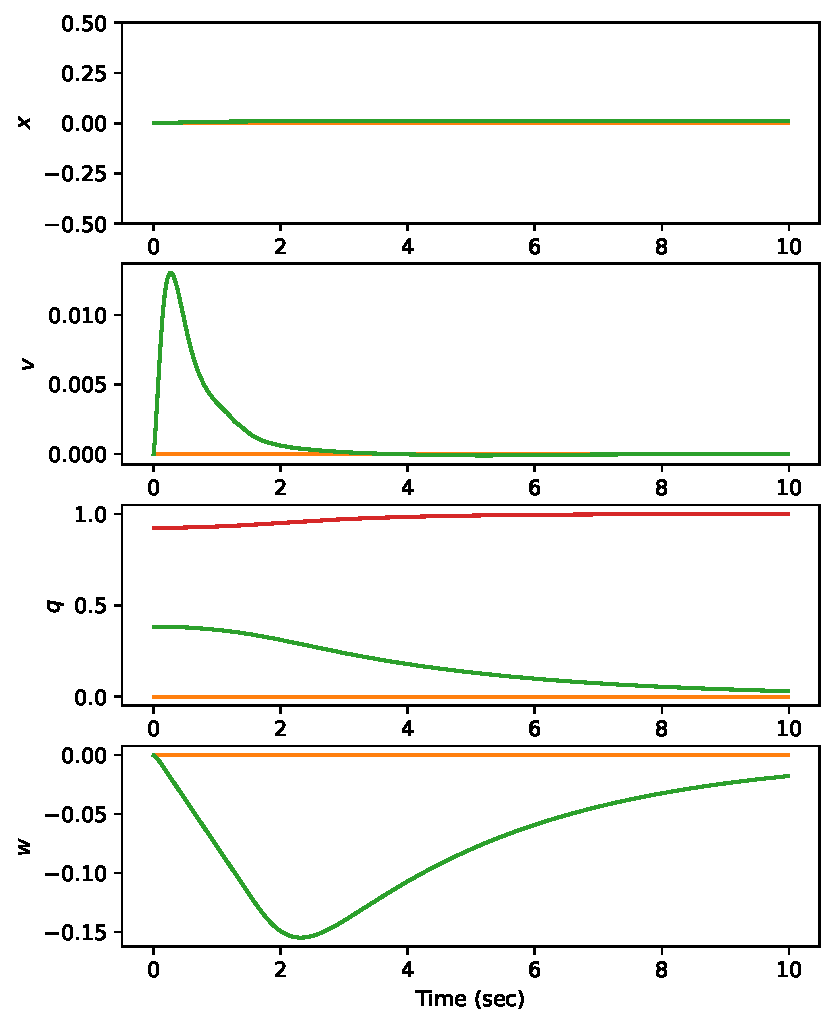
\includegraphics[width=\textwidth]{state45dz1.pdf}
		\caption{orthagonal collocation}
	\end{subfigure}%
	\begin{subfigure}[b]{0.3\textwidth}
		\centering
		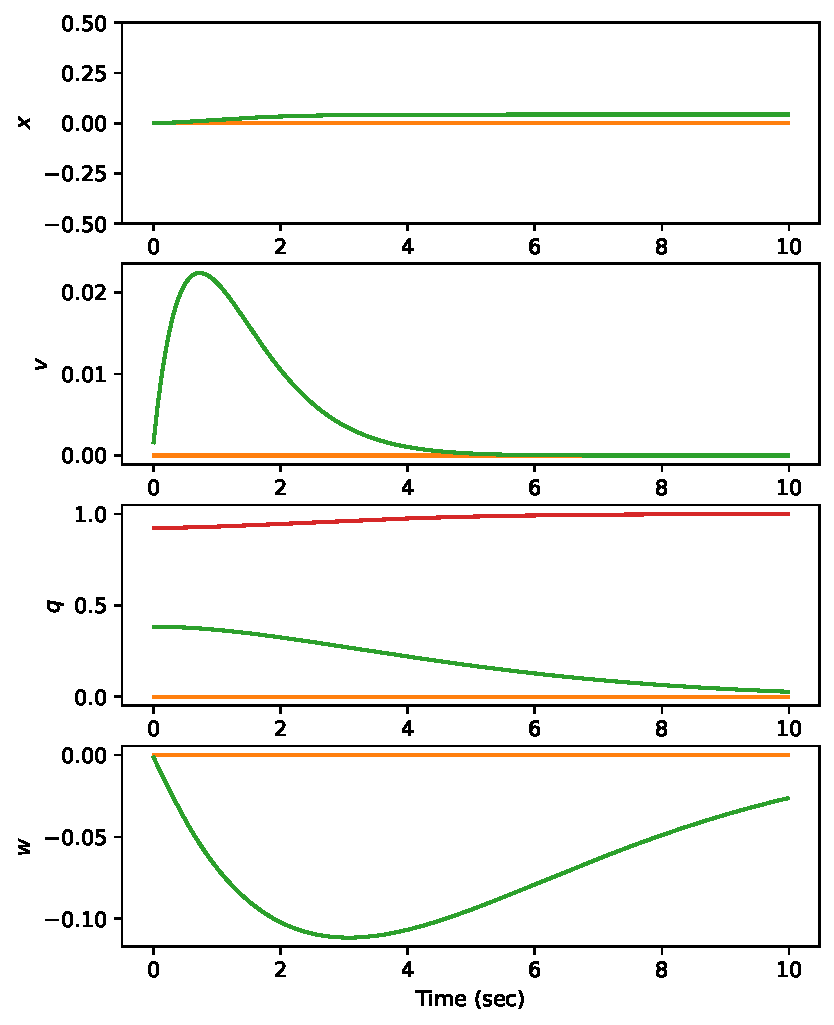
\includegraphics[width=\textwidth]{state45dz3.pdf}
		\caption{multiple shooter}
	\end{subfigure}
	\begin{subfigure}[b]{0.3\textwidth}
		\centering
		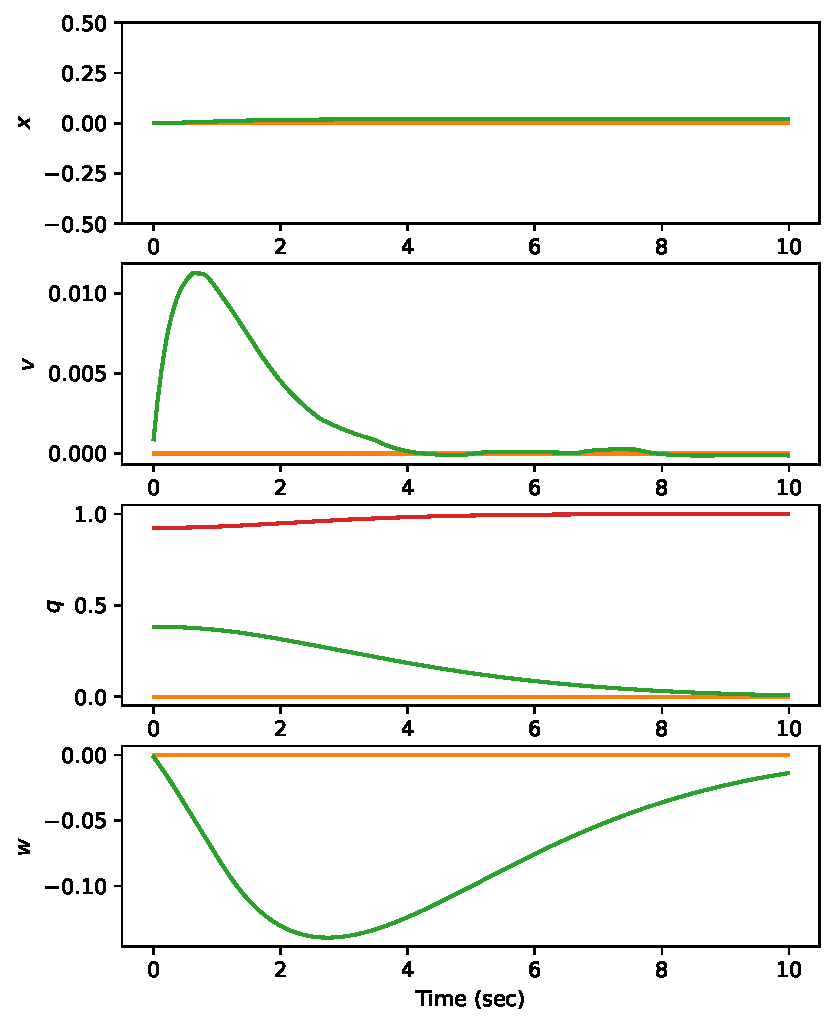
\includegraphics[width=\textwidth]{state45dz2.pdf}
		\caption{Chebyshev pseudospectral}
	\end{subfigure}
	\caption{State data on a simulation requiring a $45^{\circ}$ rotation about the $z$ axis.}
	\label{fig:state45z}
\end{figure}

\begin{figure}[H]
	\centering
	\begin{subfigure}[b]{0.3\textwidth}
		\centering
		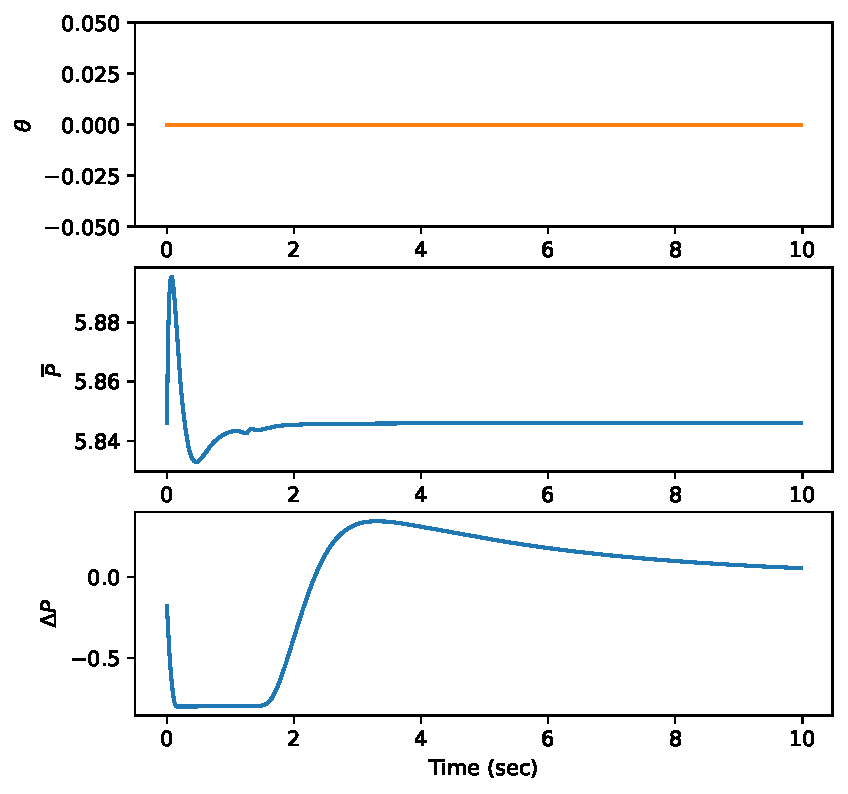
\includegraphics[width=\textwidth]{control45dz4.pdf}
		\caption{orthagonal collocation}
	\end{subfigure}%
	\begin{subfigure}[b]{0.3\textwidth}
		\centering
		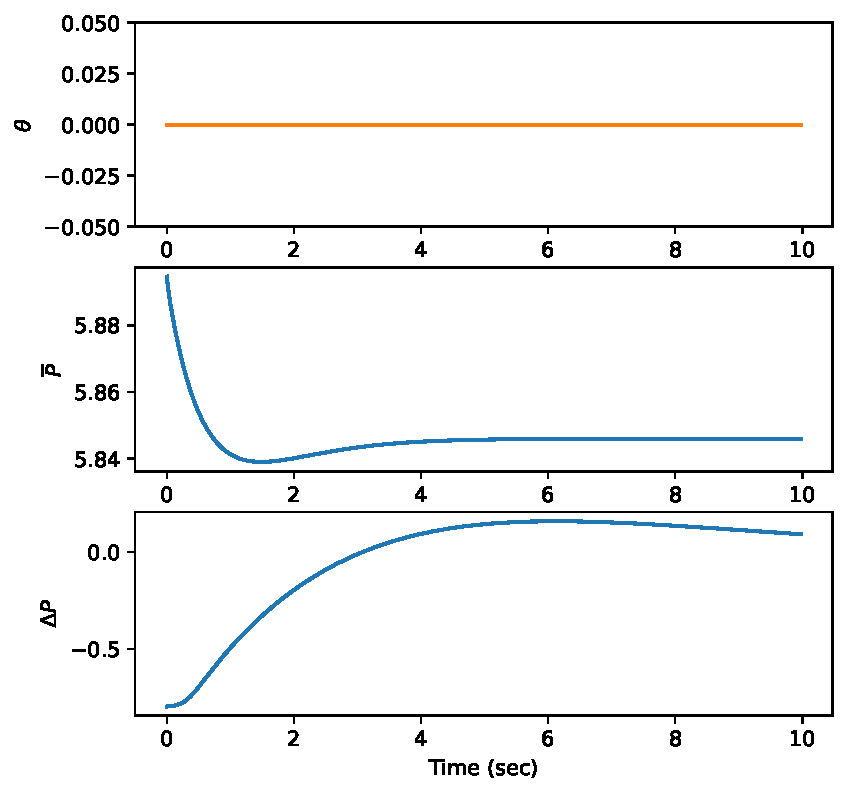
\includegraphics[width=\textwidth]{control45dz6.pdf}
		\caption{multiple shooter}
	\end{subfigure}
	\begin{subfigure}[b]{0.3\textwidth}
		\centering
		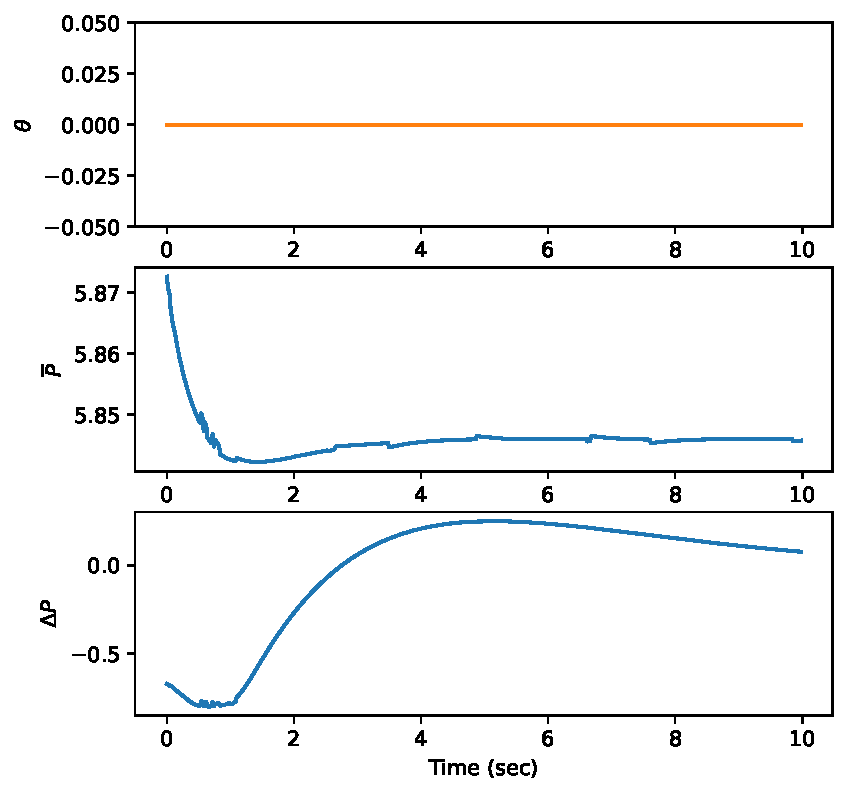
\includegraphics[width=\textwidth]{control45dz5.pdf}
		\caption{Chebyshev pseudospectral}
	\end{subfigure}
	\caption{Control data on a simulation requiring a $45^{\circ}$ rotation about the $z$ axis.}
	\label{fig:control45z}
\end{figure}


\begin{figure}[H]
	\centering
	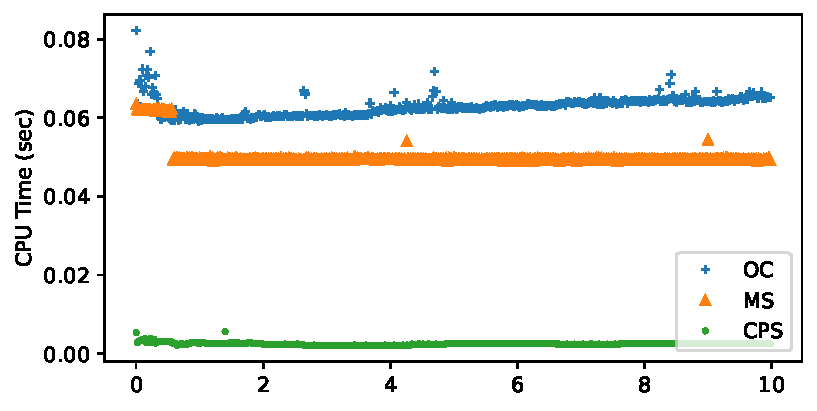
\includegraphics[width=\textwidth]{time45dz.pdf}
	\caption{CPU time for simulation requiring a $45^{\circ}$ rotation about the $z$ axis.}
	\label{fig:kfangle}
\end{figure}


\begin{figure}[H]
	\centering
	\begin{subfigure}[b]{0.3\textwidth}
		\centering
		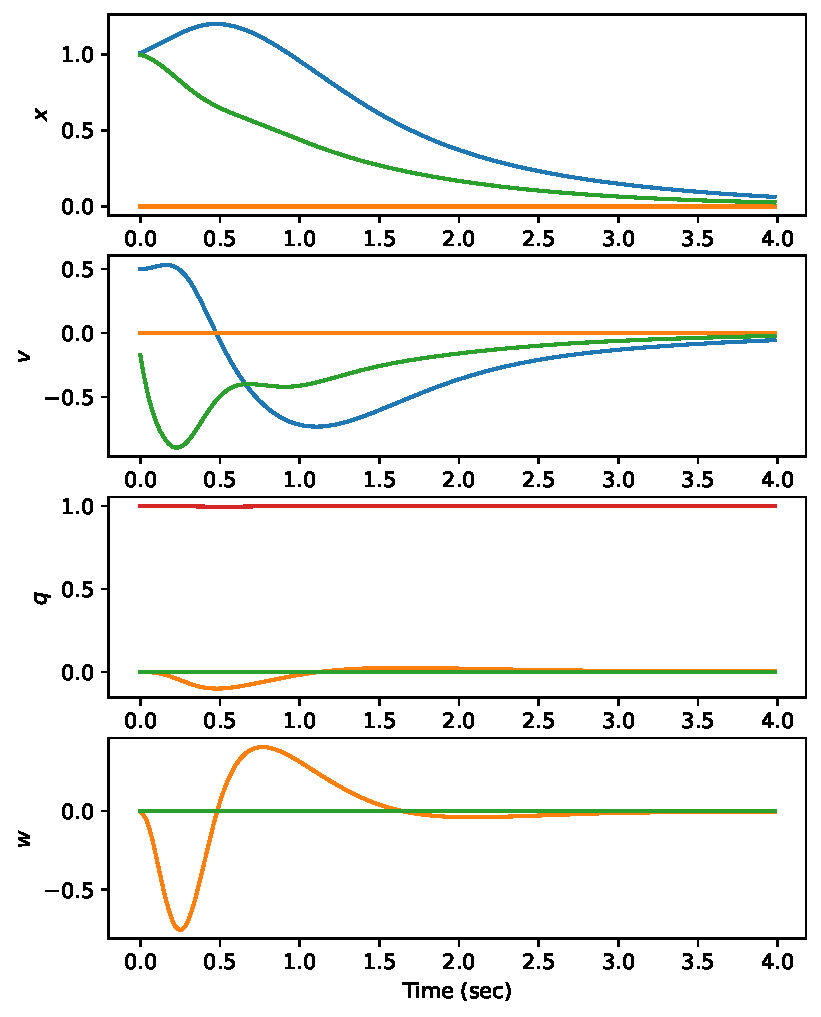
\includegraphics[width=\textwidth]{statex1z1vx1.pdf}
		\caption{orthagonal collocation}
	\end{subfigure}%
	\begin{subfigure}[b]{0.3\textwidth}
		\centering
		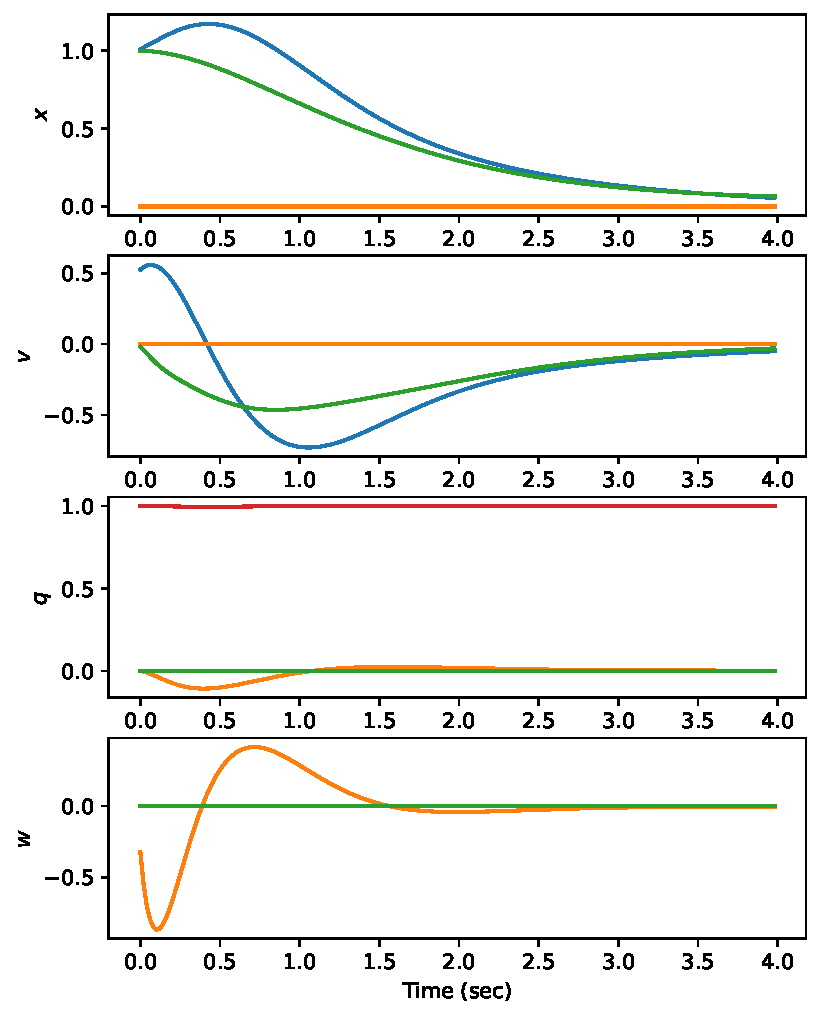
\includegraphics[width=\textwidth]{statex1z1vx3.pdf}
		\caption{multiple shooter}
	\end{subfigure}
	\begin{subfigure}[b]{0.3\textwidth}
		\centering
		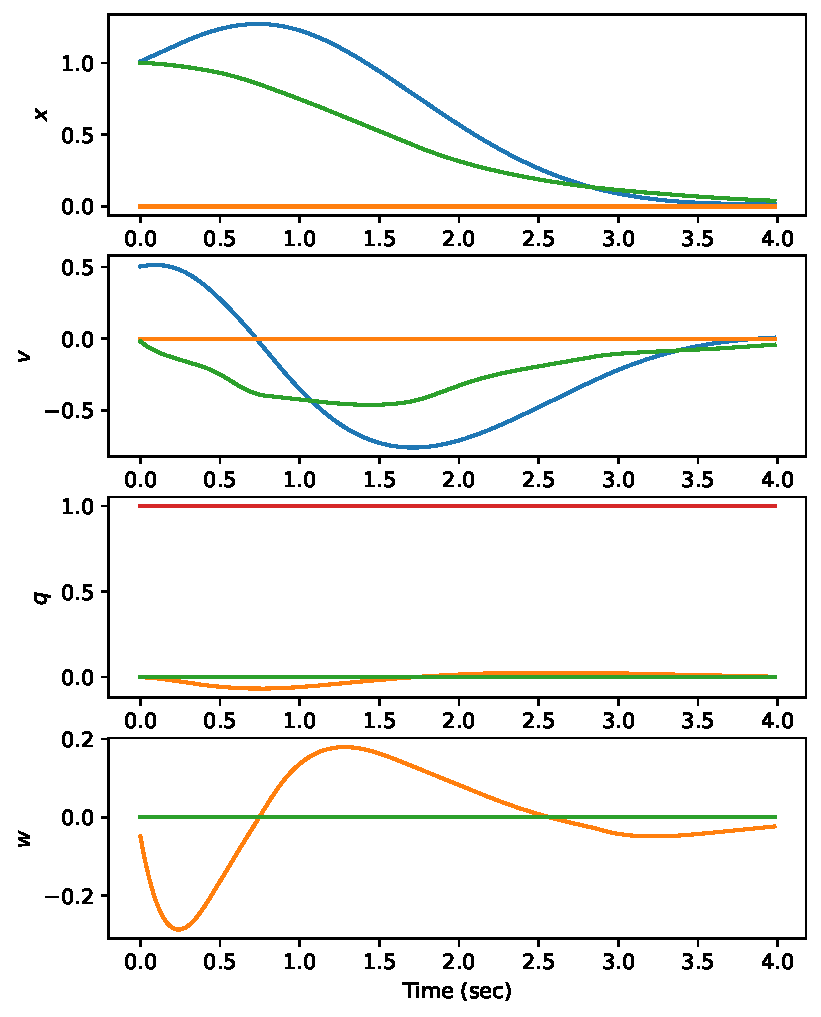
\includegraphics[width=\textwidth]{statex1z1vx2.pdf}
		\caption{Chebyshev pseudospectral}
	\end{subfigure}
	\caption{State data on a simulation with initial conditions: $x = 1$, $z=1$, $v_x = 0.5$ }
	\label{fig:state45z}
\end{figure}

\begin{figure}[H]
	\centering
	\begin{subfigure}[b]{0.3\textwidth}
		\centering
		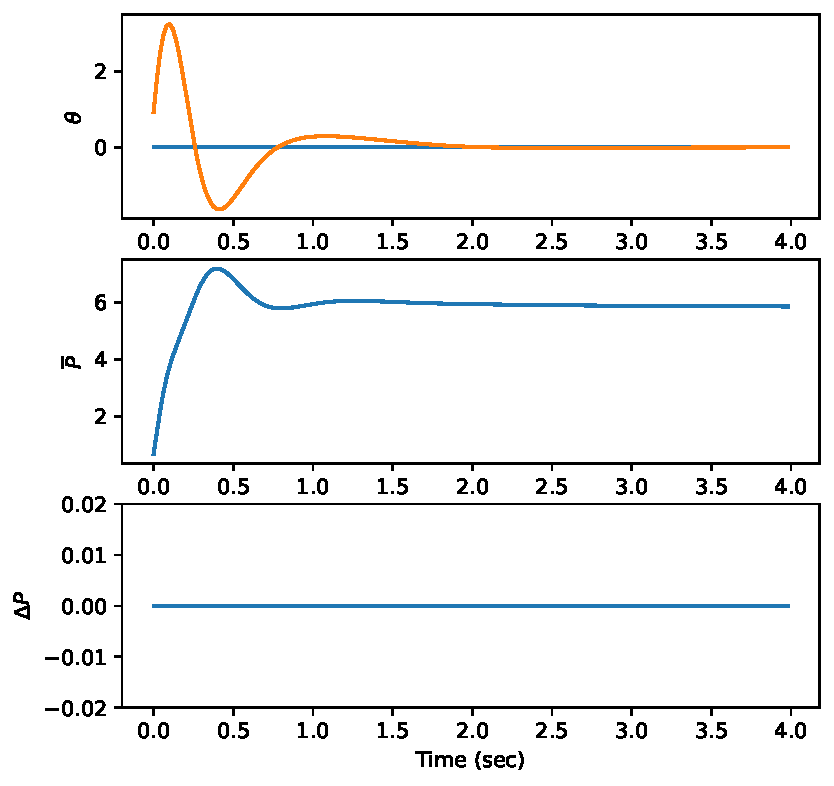
\includegraphics[width=\textwidth]{controlx1z1vx4.pdf}
		\caption{orthagonal collocation}
	\end{subfigure}%
	\begin{subfigure}[b]{0.3\textwidth}
		\centering
		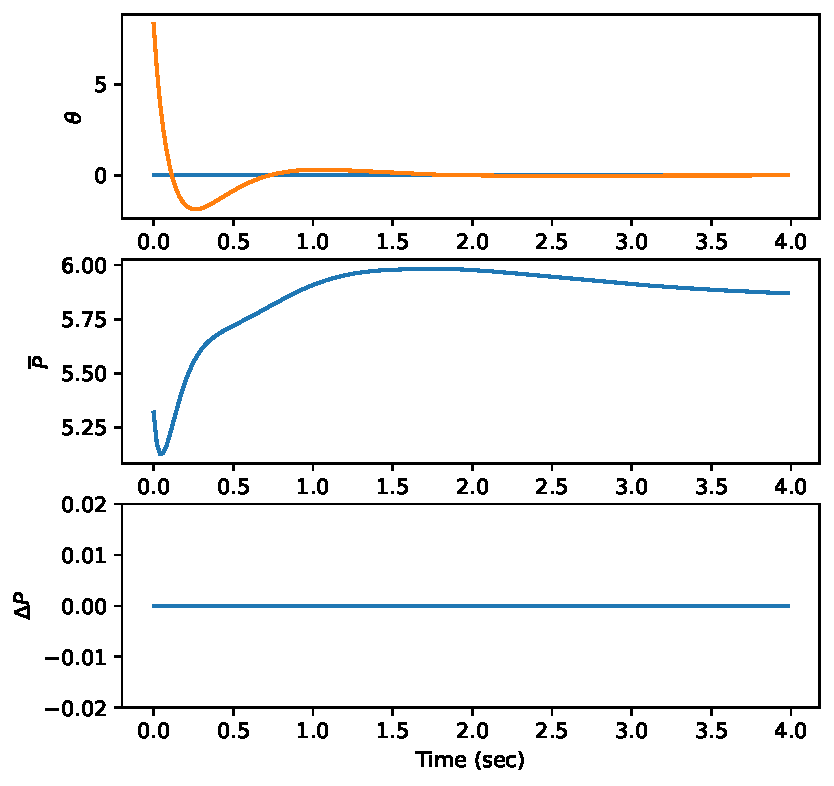
\includegraphics[width=\textwidth]{controlx1z1vx6.pdf}
		\caption{multiple shooter}
	\end{subfigure}
	\begin{subfigure}[b]{0.3\textwidth}
		\centering
		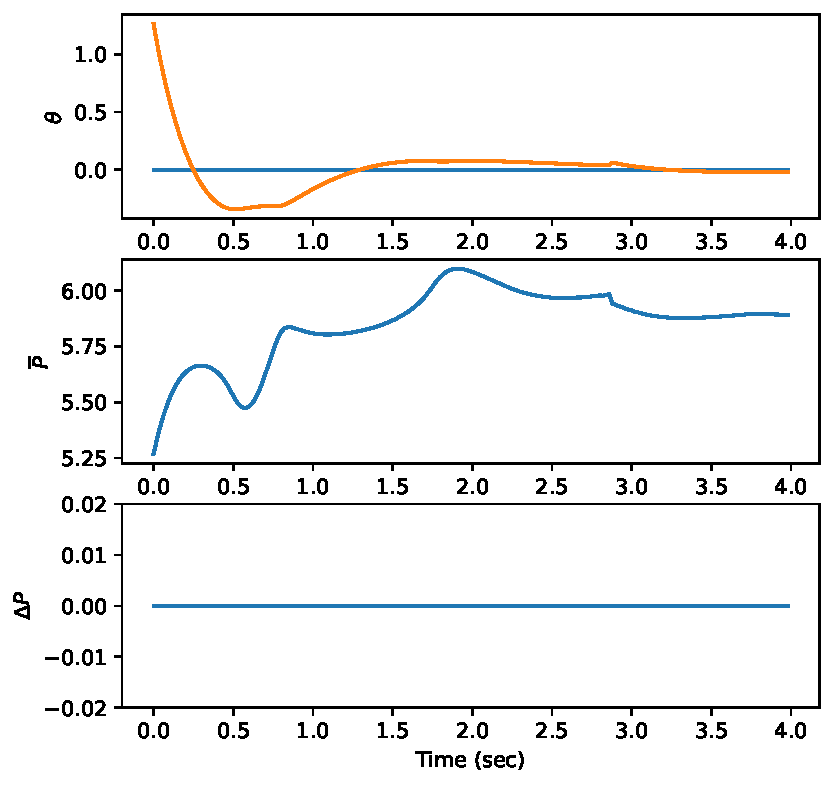
\includegraphics[width=\textwidth]{controlx1z1vx5.pdf}
		\caption{Chebyshev pseudospectral}
	\end{subfigure}
	\caption{Control data on a simulation with initial conditions: $x = 1$, $z=1$, $v_x = 0.5$}
	\label{fig:control45z}
\end{figure}


\begin{figure}[H]
	\centering
	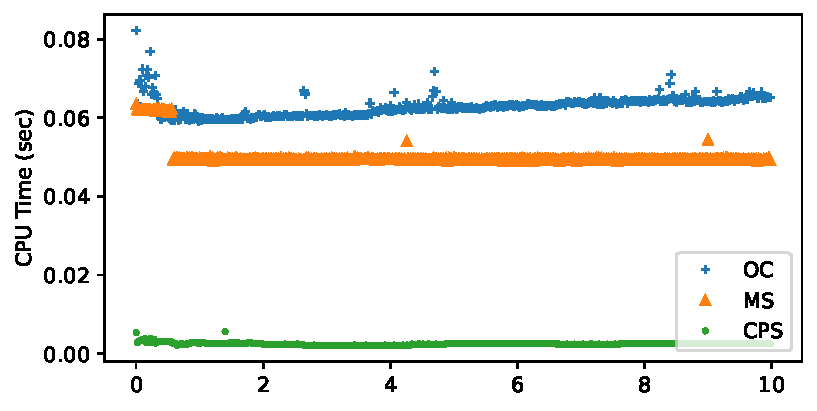
\includegraphics[width=\textwidth]{time45dz.pdf}
	\caption{CPU time for a simulation with initial conditions: $x = 1$, $z=1$, $v_x = 0.5$}
	\label{fig:timex1z1vx}
\end{figure}

\begin{figure}[H]
	\centering
	\begin{subfigure}[b]{0.3\textwidth}
		\centering
		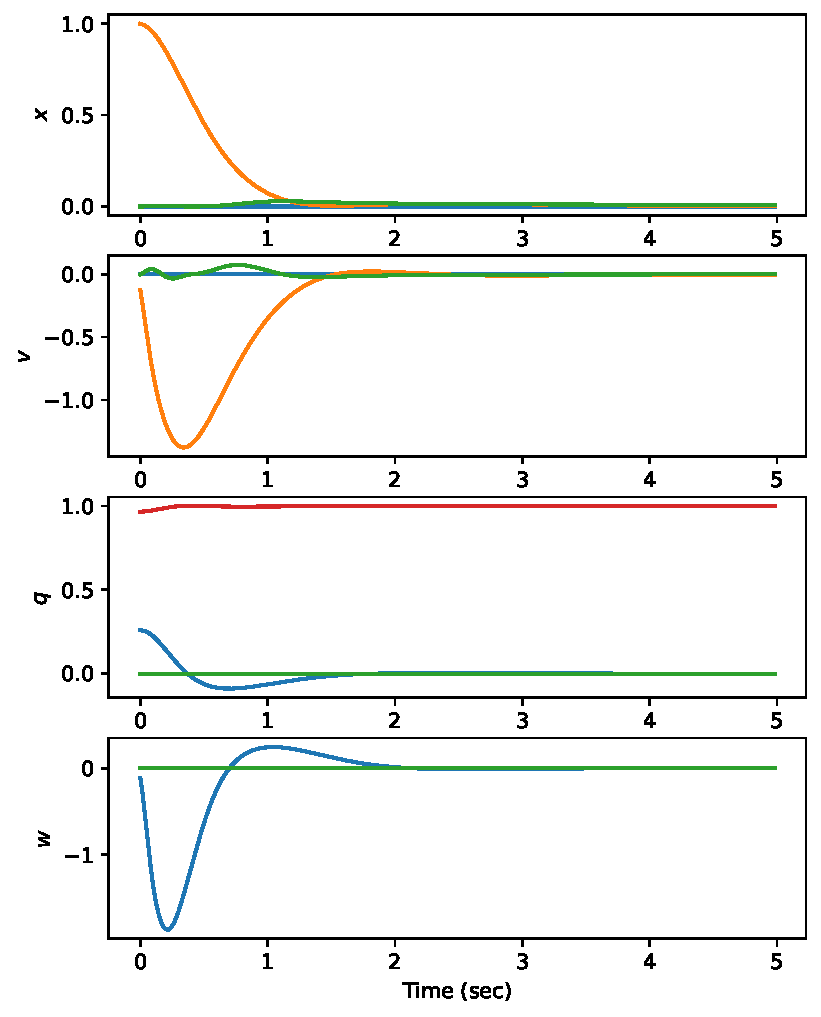
\includegraphics[width=\textwidth]{statey115dx1.pdf}
		\caption{orthagonal collocation}
	\end{subfigure}%
	\begin{subfigure}[b]{0.3\textwidth}
		\centering
		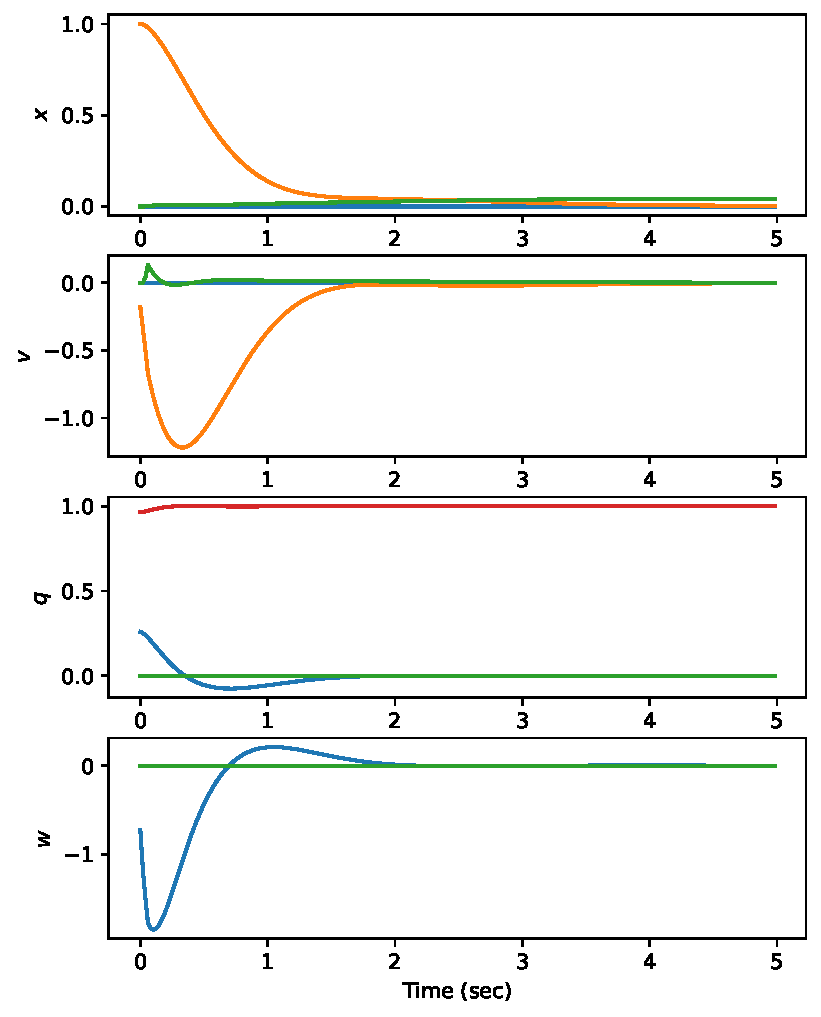
\includegraphics[width=\textwidth]{statey115dx3.pdf}
		\caption{multiple shooter}
	\end{subfigure}
	\begin{subfigure}[b]{0.3\textwidth}
		\centering
		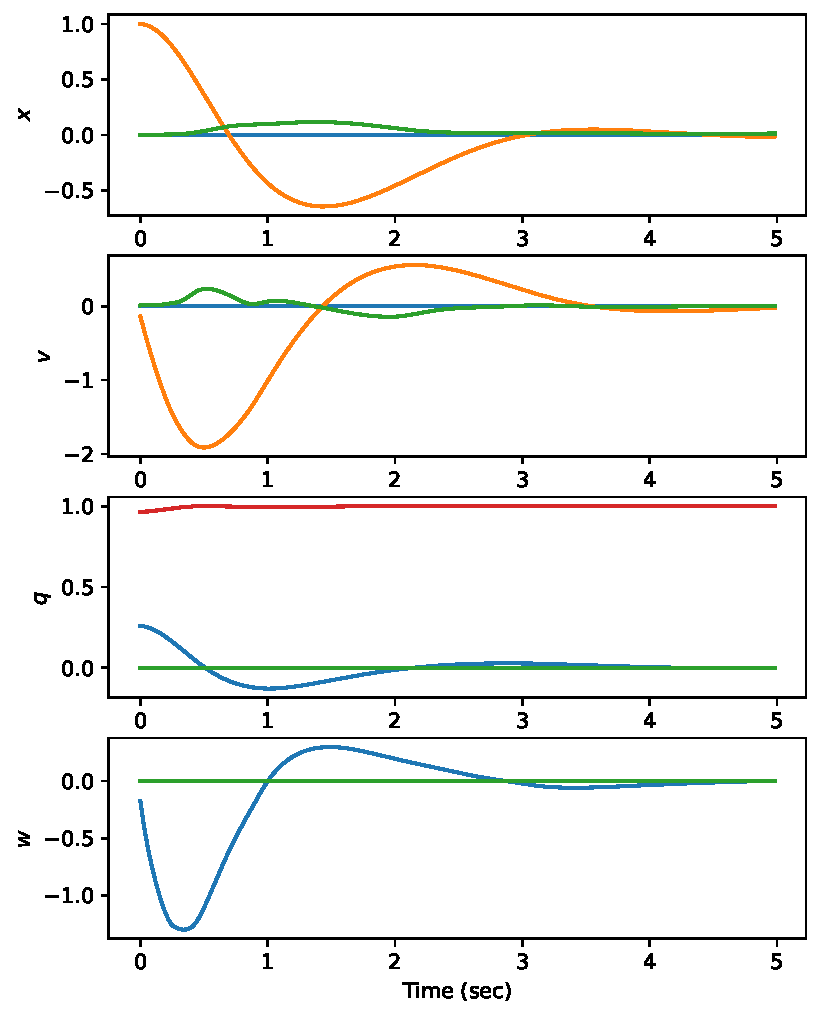
\includegraphics[width=\textwidth]{statey115dx2.pdf}
		\caption{Chebyshev pseudospectral}
	\end{subfigure}
	\caption{State data on a simulation with initial conditions: $y = 1$,$15^{\circ}$ rotation about $x$ axis.}
	\label{fig:state45z}
\end{figure}

\begin{figure}[H]
	\centering
	\begin{subfigure}[b]{0.3\textwidth}
		\centering
		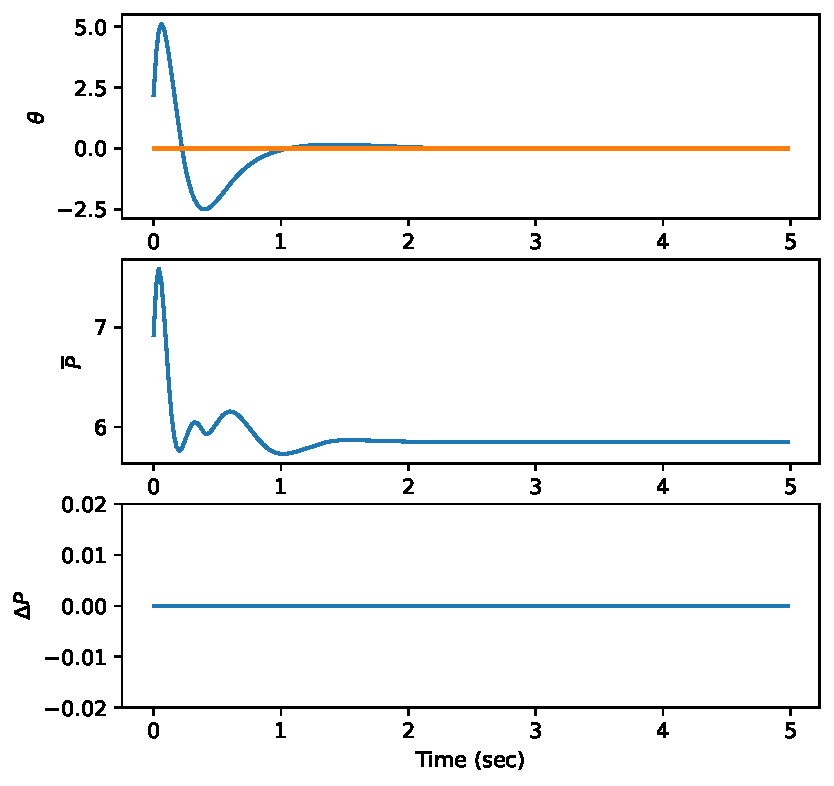
\includegraphics[width=\textwidth]{controly115dx4.pdf}
		\caption{orthagonal collocation}
	\end{subfigure}%
	\begin{subfigure}[b]{0.3\textwidth}
		\centering
		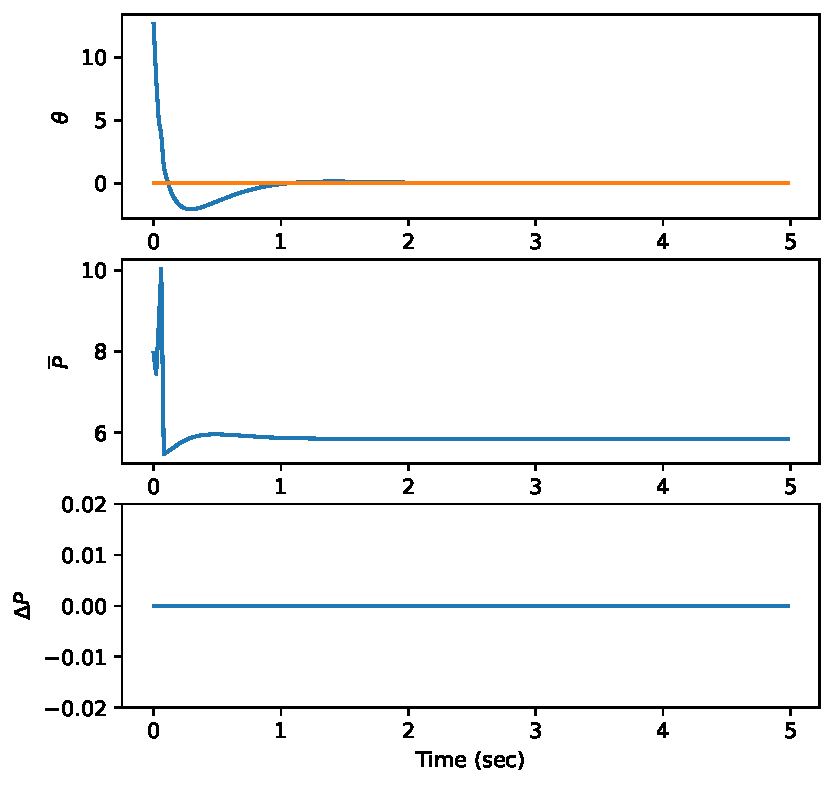
\includegraphics[width=\textwidth]{controly115dx6.pdf}
		\caption{multiple shooter}
	\end{subfigure}
	\begin{subfigure}[b]{0.3\textwidth}
		\centering
		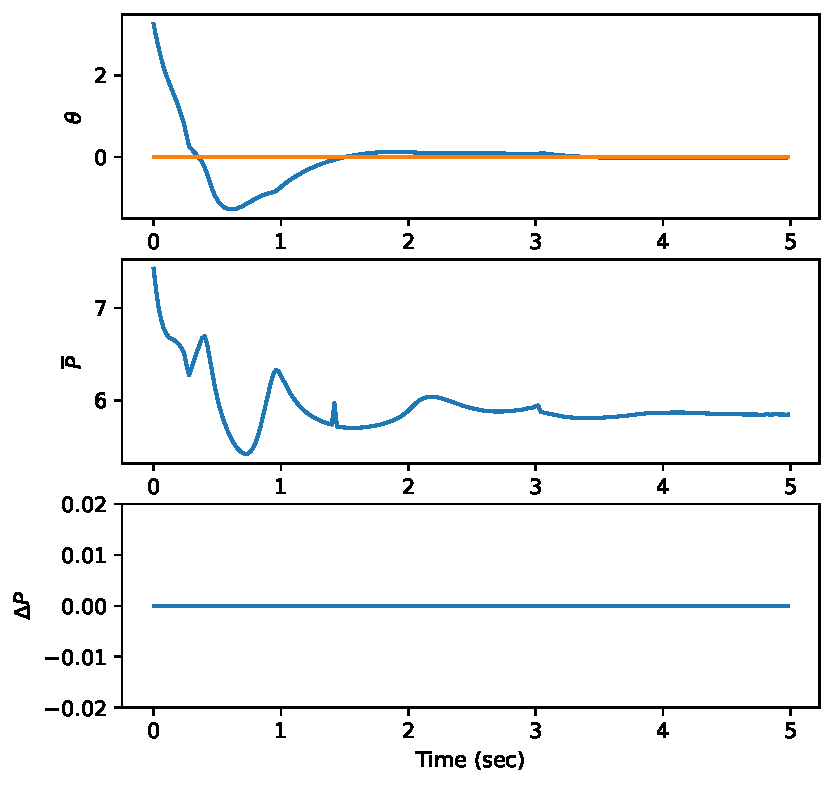
\includegraphics[width=\textwidth]{controly115dx5.pdf}
		\caption{Chebyshev pseudospectral}
	\end{subfigure}
	\caption{Control data on a simulation with initial conditions: $y = 1$,$15^{\circ}$ rotation about $x$ axis.}
	\label{fig:control45z}
\end{figure}


\begin{figure}[H]
	\centering
	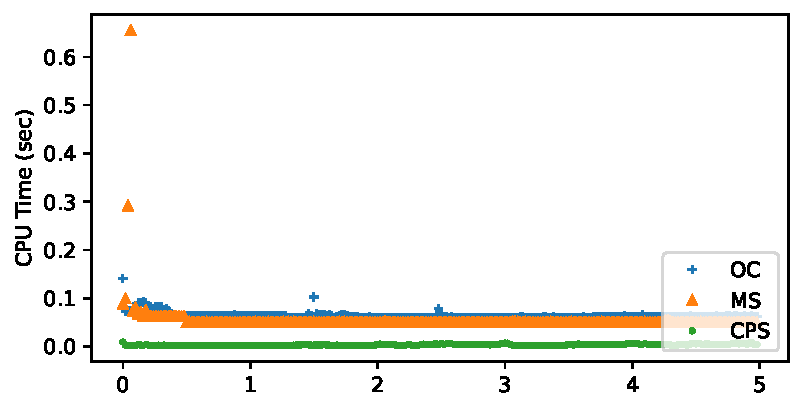
\includegraphics[width=\textwidth]{timey115dx.pdf}
	\caption{CPU time for simulation with initial conditions: $y = 1$,$15^{\circ}$ rotation about $x$ axis.}
	\label{fig:kfangle}
\end{figure}




\begin{figure}[H]
	\centering
	\begin{subfigure}[b]{0.3\textwidth}
		\centering
		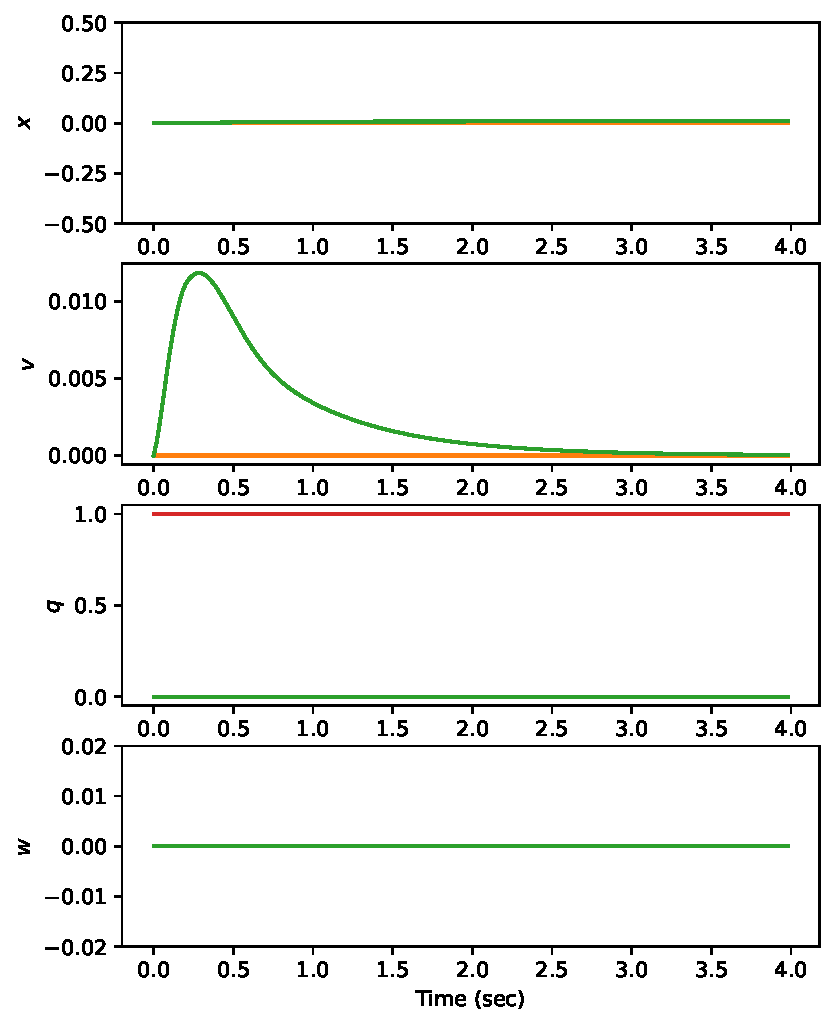
\includegraphics[width=\textwidth]{statehover1.pdf}
		\caption{orthagonal collocation}
	\end{subfigure}%
	\begin{subfigure}[b]{0.3\textwidth}
		\centering
		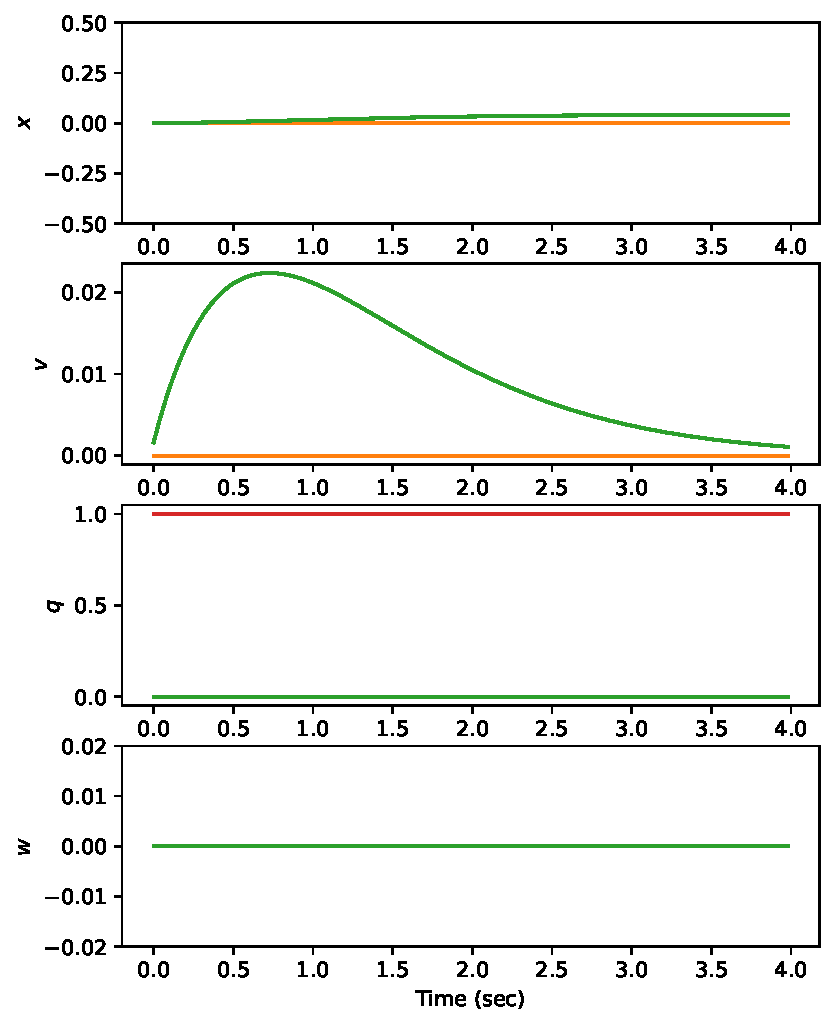
\includegraphics[width=\textwidth]{statehover3.pdf}
		\caption{multiple shooter}
	\end{subfigure}
	\begin{subfigure}[b]{0.3\textwidth}
		\centering
		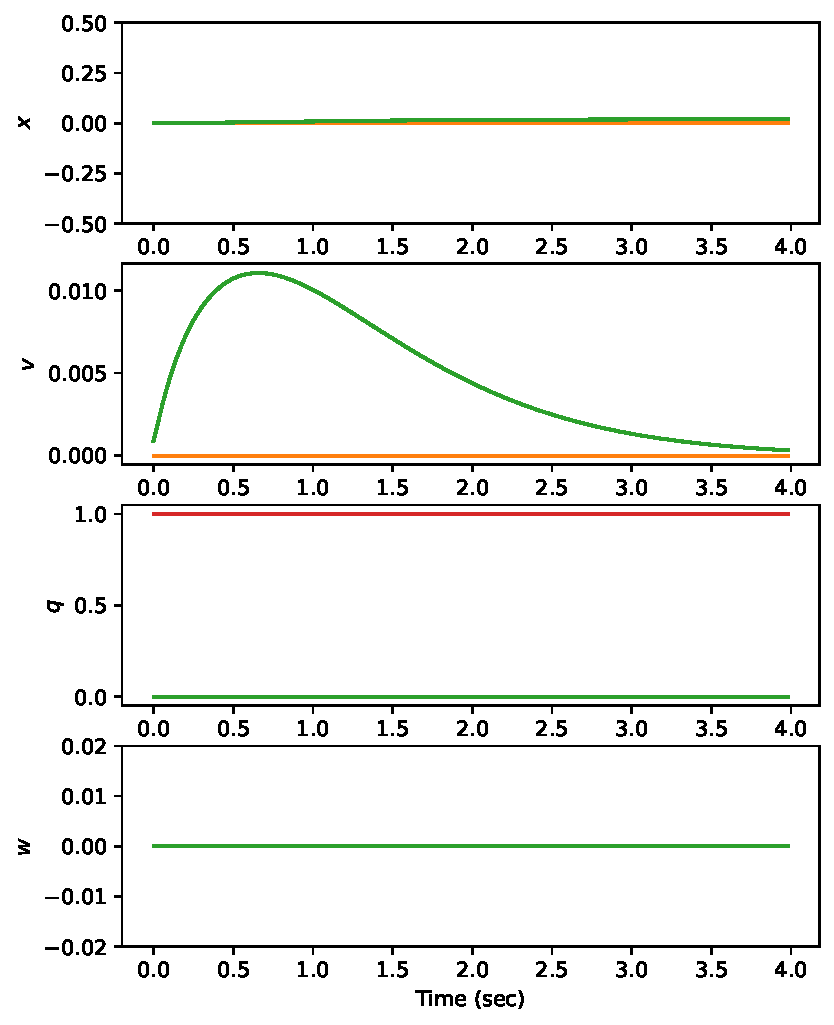
\includegraphics[width=\textwidth]{statehover2.pdf}
		\caption{Chebyshev pseudospectral}
	\end{subfigure}
	\caption{State data on a simulation with initial state equal to goal state.}
	\label{fig:state45z}
\end{figure}

\begin{figure}[H]
	\centering
	\begin{subfigure}[b]{0.3\textwidth}
		\centering
		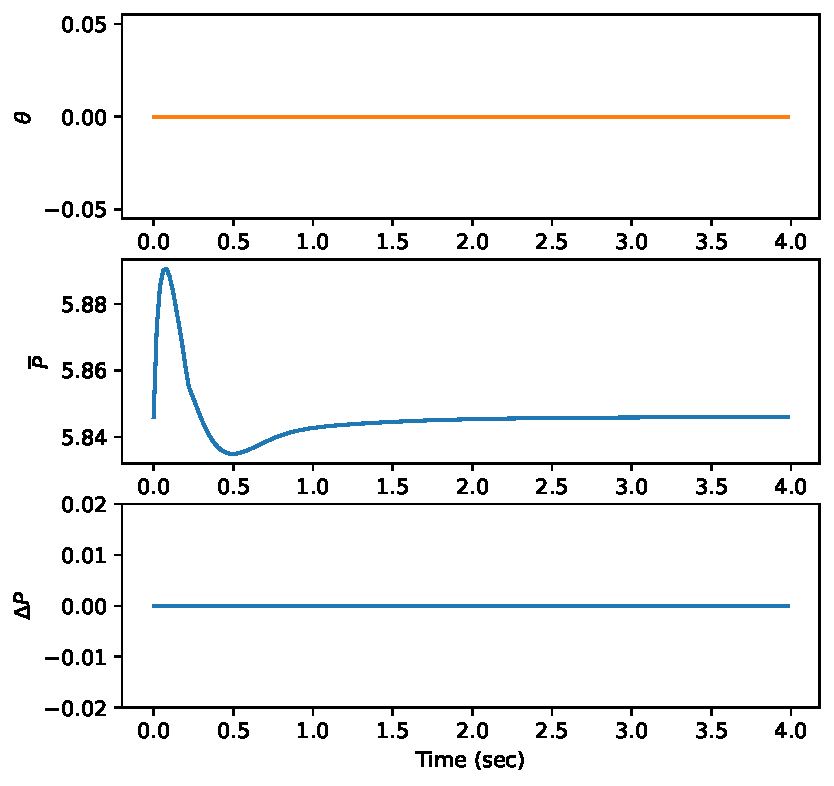
\includegraphics[width=\textwidth]{controlhover4.pdf}
		\caption{orthagonal collocation}
	\end{subfigure}%
	\begin{subfigure}[b]{0.3\textwidth}
		\centering
		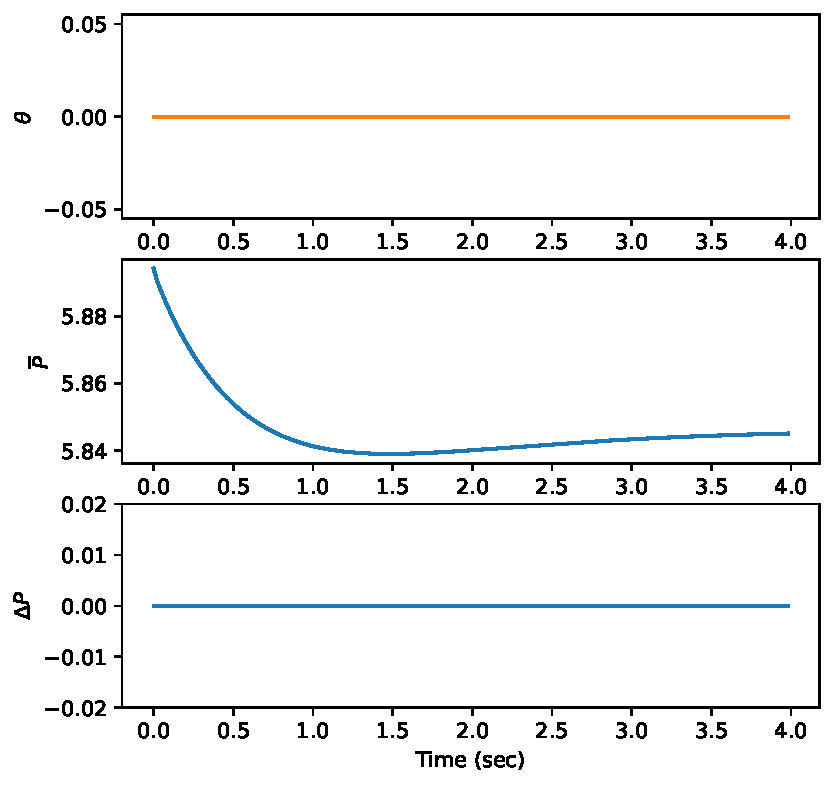
\includegraphics[width=\textwidth]{controlhover6.pdf}
		\caption{multiple shooter}
	\end{subfigure}
	\begin{subfigure}[b]{0.3\textwidth}
		\centering
		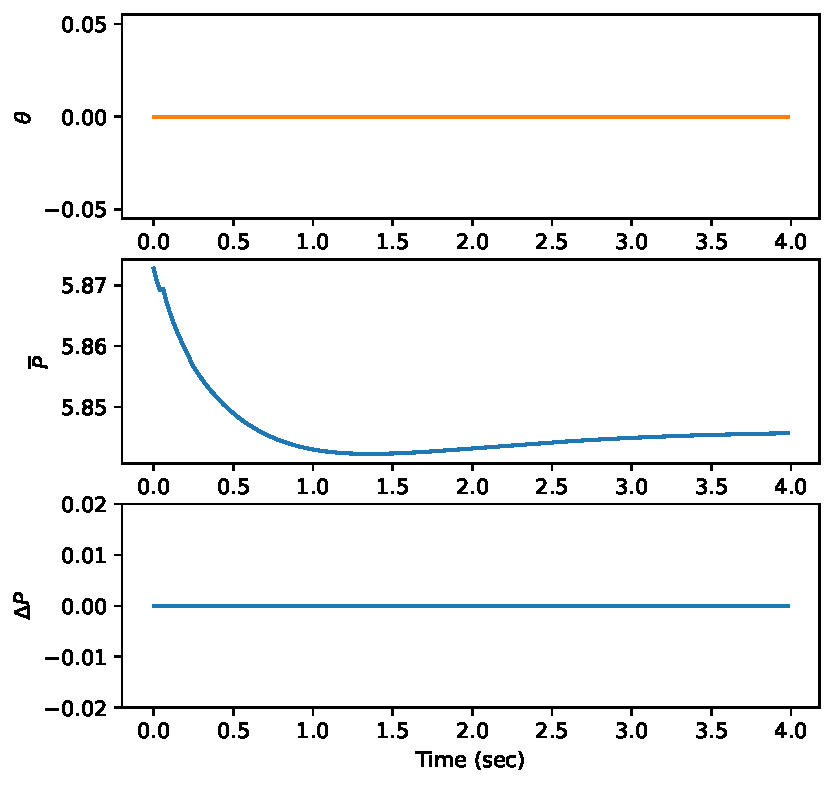
\includegraphics[width=\textwidth]{controlhover5.pdf}
		\caption{Chebyshev pseudospectral}
	\end{subfigure}
	\caption{Control data on a simulation with initial state equal to goal state.}
	\label{fig:control45z}
\end{figure}


\begin{figure}[H]
	\centering
	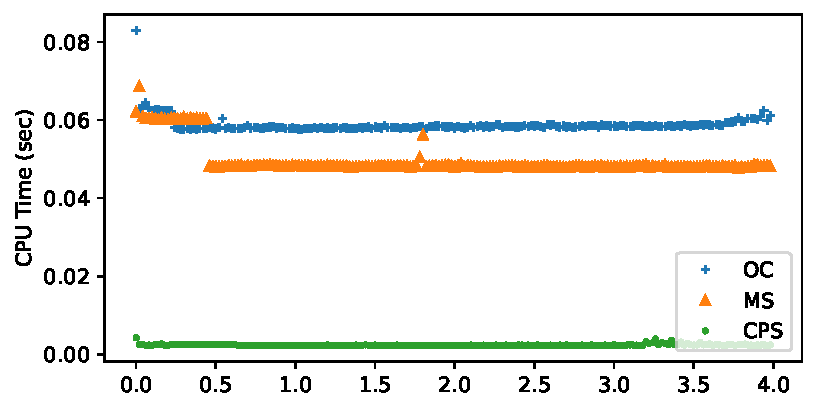
\includegraphics[width=\textwidth]{timehover.pdf}
	\caption{CPU time for simulation with initial state equal to goal state.}
	\label{fig:kfangle}
\end{figure}


\begin{table}[h!]	
	\begin{center}
		\begin{tabular}{ | l | c | c | c | } 
			\hline
			initial state & OC  & MS & CPS \\
			\hline
			$45^{\circ}$ rotation about $z$ axis & 0.063 &       0.056 & 0.002 \\ 
			$x = 1$, $z=1$, $v_x = 0.5$  & 0.059          &        0.046 & 0.003 \\ 
			$y = 1$,$15^{\circ}$ rotation about $x$ axis &0.063          &       0.06 & 0.004\\ 
				initial state equal to goal state & 0.062    &            0.056  & 0.002 \\ 
			\hline
		\end{tabular}
		\caption{Comparison of average CPU time in seconds for solution of NLP for a series of  simulations. Methods include orthagonal collocation (OC),  multiple shooter (MS), and Chebyshev pseudospectral method (CPS). }
	\end{center}
\end{table}

Our goal is to run our control algorithm at $50$Hz on the raspberry Pi 5. The CPU speed of the Pi is 2.4GHz while our experiments were run on a machine with a CPU speed of 3.49GHz. To meet our goal of 50Hz on the Pi we need a solution time on the experiment machine of less than $0.014$ seconds.
	\section*{Conclusions}
	
	
	
%	\nocite{*}
%	
\bibliographystyle{annotate}
\bibliography{references.bib}
\end{document}

